\documentclass[12pt, a4paper, twoside, openright]{book}

\usepackage{apacite}
\usepackage{doi}
\usepackage{nomencl}

\usepackage[acronym]{glossaries}

\usepackage{caption}
\usepackage{subcaption}

\usepackage[T1]{fontenc}
\usepackage{wrapfig}
\usepackage[figuresright]{rotating}

\usepackage{vuw_thesis} % sets up some local things, mostly the front page

\usepackage{natbib}
\setcitestyle{authoryear, open={(},close={)}}

\usepackage{palatino} % sets palatino as the default font
\usepackage{amsmath}
\usepackage{url} % for typesetting urls
\usepackage{graphicx}
\usepackage{lscape}
\usepackage{hhline}
\usepackage{caption}
\captionsetup{width=1\linewidth, font=footnotesize}
\usepackage{threeparttable}
\usepackage{multirow}
\usepackage{longtable}
\usepackage[compact]{titlesec}
\usepackage{booktabs}
\usepackage{tabularx}
\usepackage{ltablex}
\usepackage{float}
\usepackage{multicol}
\usepackage{placeins}
\usepackage{hanging}
\usepackage{fancyhdr}
\usepackage{placeins}

\usepackage{array}
\newcolumntype{L}[1]{>{\raggedright\let\newline\\\arraybackslash\hspace{0pt}}m{#1}}
\newcolumntype{C}[1]{>{\centering\let\newline\\\arraybackslash\hspace{0pt}}m{#1}}
\newcolumntype{R}[1]{>{\raggedleft\let\newline\\\arraybackslash\hspace{0pt}}m{#1}}

\setlength{\parindent}{0pt}

\setlength{\headheight}{24pt}

\usepackage[inner=3.3cm,outer=2.5cm,top=2.9cm,bottom=2.9cm]{geometry}

\usepackage{hyperref}

\hypersetup{colorlinks=false, linkcolor=blue, filecolor=black, urlcolor=black, citecolor=black, linktocpage,}

\newcommand{\citemulti}[1]{\citeauthor{#1}, \citeyear{#1}}

 %Include the bibliogaphy in the word count
%TC:incbib

%Include in-text citations in the word count
%TC:macro \cite [option:text,text]
%TC:macro \citep [option:text,text]
%TC:macro \citet [option:text,text]

%Include tables in the word count
%TC:group table 0 1
%TC:group tabular 1 1
 

\pagestyle{fancy}
% with this we ensure that the chapter and section headings are in lowercase.
\renewcommand{\chaptermark}[1]{%
    \markboth{}{}}
%    \renewcommand{\sectionmark}[1]{%
%    \markright{\thesection\ #1}}
    \fancyhf{}  % delete current header and footer
    \fancyhead[LO,RE]{\bfseries\thepage}
    \fancyhead[LE]{\emph\textit{\nouppercase{\rightmark}}}
    \fancyhead[RO]{\emph\textit{\nouppercase{\leftmark}}}
    \fancyhead[RE]{}
    \fancyhead[LO]{}
    \fancyfoot[CE]{\emph\textit{\nouppercase{\rightmark}}}
    \fancyfoot[CO]{\emph\textit{\nouppercase{\leftmark}}}
    \fancyfoot[CE]{\thepage}
    \fancyfoot[CO]{\thepage}
    \renewcommand{\headrulewidth}{0.5pt}
    \renewcommand{\footrulewidth}{0.5pt}
    \addtolength{\headheight}{3pt} % space for the rule
    \fancypagestyle{plain}{%
    \fancyhead{} % get rid of headers on plain pages
    \renewcommand{\headrulewidth}{0pt} % and the line
}

\begin{document}
\setlength{\parskip}{8pt}
%\normallinespacing
\frontmatter
% % Book style knows about front matter

% % Report style doesn't so you need to set roman numbering etc yourself :-(

 

\title{Earth-shattering research}

\author{Me}

\subject{Geophysics}

% If MSC thesis
\mscthesisonly
% If PhD thesis
% \phd

\maketitle

\clearpage{\pagestyle{empty}\clearpage}
\clearpage{\pagestyle{empty}\cleardoublepage}

\cleardoublepage 
\chapter{Abstract}

I did some cool science and worked some things out.


 

%\addcontentsline{toc}{chapter}{Abstract}


\cleardoublepage
\chapter{Acknowledgements}

Remember to acknowledge people who helped you (in the field, in the lab, in life, your supervisors). Acknowledge your funders and data providers. And anyone else you want.


%\addcontentsline{toc}{chapter}{Acknowledgements}

\clearpage{\pagestyle{empty}\cleardoublepage}

\newpage
\phantomsection
\cleardoublepage 
\cleardoublepage

\addcontentsline{toc}{chapter}{\contentsname}
\tableofcontents
\newpage
\phantomsection
\cleardoublepage

\addcontentsline{toc}{section}{List of figures}
\listoffigures
\newpage
\phantomsection
\cleardoublepage

\addcontentsline{toc}{section}{List of tables}
\listoftables
\newpage
\phantomsection
\cleardoublepage

%\addcontentsline{toc}{section}{List of acronyms}
%\include{Acronyms}
%\newpage
%\phantomsection
%\cleardoublepage

%%%%%%%%%%%%%%%%%%%%%%%%%%%%%%%%%%%%%%%%%%%%%%%%%%%%%%%

 

% book style knows about mainmatter
% if you are using report style you will have to rest page numbering etc.
\mainmatter
\pagestyle{fancy}

%%%%%%%%%%%%%%%%%%%%%%%%%%%%%%%%%%%%%%%%%%%%%%%%%%%%%%%

% Include your chapters here 

\chapter{Introduction}

Your work here. Cite people using either inline:~\citet{Hopkins2021213} or not:~\citep{Hopkins2021213}.
Reference figures, tables and sections like: Figure~\ref{fig:tectonic_setting}, Table:~\ref{tab:study_period_events}, Section~\ref{example}. 
Remember that all units and quantities should be separated using a non-breaking half-space: 7\,km


\section{Example figure and table}\label{example}

\begin{figure}

    \centering

    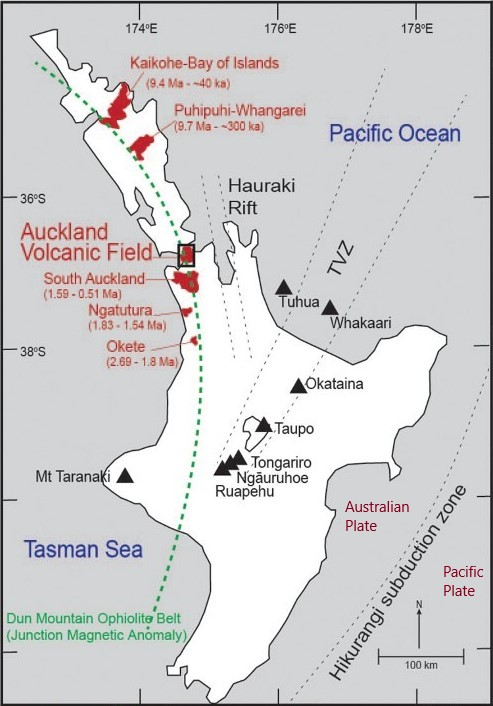
\includegraphics[width=0.9\textwidth]{./Figures/Hopkins2021Fig1Av2.jpg}

    \centering

    \caption[Short caption for ToC]{Big caption}
    \label{fig:tectonic_setting}

\end{figure}


\begin{table}
    \centering
    \caption[Short caption for ToT]{Table captions go above the table}
    \begin{tabular}{c|c|c|c|c}
        Year & Total Events & EQ & QB & Unlabelled \\
        \hline
        2011 & 45 & 13 & 32 & 0 \\
    \end{tabular}
    \label{tab:study_period_events}
\end{table}





%%%%%%%%%%%%%%%%%%%%%%%%%%%%%%%%%%%%%%%%%%%%%%%%%%%%%%%

% and of course book style knows about backmatter

% \backmatter

% and of course report style doesn't

\cleardoublepage
\phantomsection

% $$$$$$$$$$$$$$$$$  Reference style  Starts $$$$$$$$$$$$$$


%	\renewcommand*\bibname{\centerline{REFERENCES}} 
\addcontentsline{toc}{chapter}{References}
	\newcommand{\BIBdecl}{\setlength{\itemsep}{0pt}}%To control space between bibliography entries
    \bibliographystyle{plainnat}
	\bibliography{refs}

% $$$$$$$$$$$$$$$$$  Reference style Ends  $$$$$$$$$$$$$$

\cleardoublepage

% \include{Appendix}


\end{document}
